\documentclass[12pt]{article}
\usepackage[utf8]{inputenc}
\usepackage{amsmath}
\usepackage{graphicx}
\usepackage{xcolor}
\usepackage{geometry}
\usepackage{enumitem}
\usepackage{fancyhdr}
\usepackage{titling}
\usepackage{float}
\renewcommand{\figurename}{Gráfico}  

\geometry{letterpaper, margin=1in}
\fancypagestyle{firststyle}{
    \fancyhf{}
    \lhead{
\includegraphics[height=5cm]{../imagenes/logo.png}}
    \renewcommand{\headrulewidth}{0pt}
    }
    \pagestyle{plain}
    
    \definecolor{rojoudp}{RGB}{210,35,42}
\newcommand{\subrayadoRojo}[1]{{\color{rojoudp}\underline{\textcolor{black}{#1}}}}
\newcommand{\formulasection}[2]{%
    \vspace{1em}
    \noindent
    {\large\bfseries\color{blue}#1}\\[-4em]
    \begin{center}
        \large
      \[
      #2
      \]
    \end{center}
    \vspace{1em}
}
\setlength{\droptitle}{-3em}
\begin{document}
\begin{figure}
    \vspace{-5em}    
    \flushright
    
\includegraphics[height=4cm]{../imagenes/logo.png}\\[-3em]
\end{figure}
\begin{center}
    {\LARGE \textbf{Ayudantía Nº3: Árboles binomiales}}\\[0.5em]
    Curso: Instrumentos Derivados\\
    Profesor: Francisco Rantul\\
    Ayudante: Mateo Canales\\
\end{center}
\vspace{1pt}
{\color{rojoudp}\hrule height 2pt}
\vspace{10pt}

\section*{\subrayadoRojo{Pregunta 1}}
El precio de una acción es de \$100. En 6 meses más se espera que suba o baje un 10 \%.
La tasa libre de riesgo es del 8 \% anual continua. 


\begin{enumerate}[label=\textbf{\alph*)}]
    \item	¿Cuál es el valor de una opción call europea de 1 año con strike Price $ K = \$100 $?
    \item	¿Cuál es el valor de una opción put europea de 1 año con strike Price $ K = \$100 $?
    \item   Verifique que se cumple la paridad Put-Call
\end{enumerate}

\section*{\subrayadoRojo{Pregunta 2}}
El precio de una acción es de \$50. En 2 meses más podría valer \$53 o \$48. La tasa libre de riesgo es del 10\%
anual continua. Calcule el valor de una opción call europea de 2 meses con strike Price K=\$49. 
Considere un árbol de un solo paso.  

\begin{enumerate}[label=\textbf{\alph*)}]
    \item	Valorice la opción call europea usando argumentos de no arbitraje. 
    \item	Valorice la opción call europea usando probabilidades neutrales al riesgo.
\end{enumerate}


\section*{\subrayadoRojo{Pregunta 3}}
El precio de una acción es de \$40. Cada 3 meses se espera que suba o baje un 10\%.
La tasa libre de riesgo es de 12\% anual continua. 

\begin{enumerate}[label=\textbf{\alph*)}]

    \item	Calcule el valor de una opción put europea a 6 meses con strike Price $K=42$.
    \item   Calcule una opción put americana a 6 meses con strike Price $K=42$.
    \item   Explique la razón en la diferencia del valor respecto a la opción europea.

\end{enumerate}

\section*{\subrayadoRojo{Pregunta 4}}
Los saltos temporales de una opción son de 1 mes ($\Delta_t=\frac{1}{12}$), la tasa de interés libre de riesgo 
local es del 5\% continua anual y la tasa libre de riesgo extranjera es del 8\% continua anual. 
La volatilidad es del 12\% anual.

\begin{enumerate}[label=\textbf{\alph*)}]
    \item   Calcule u, d y p cuando se construye un árbol binomial para divisas. 
    \item   Replique el \textit{Gráfico 1}. Dónde incluya 1000 posibles trayectorias de la divisa en R o pythom, usando $S_0=1,1$ y 50 saltos de $\Delta_t=1$. {\footnotesize(\textbf{Nota:} Use set.seed(123) o similar)}
    \item   A que distribución tienden los precios si aumentamos la cantidad de saltos a 500. 
\end{enumerate}

\begin{figure}[H]
    \centering
    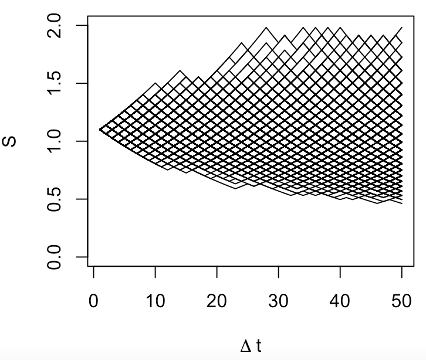
\includegraphics[height=20em]{../imagenes/Imagen 1.png}
    \caption{\textbf{Opción en el tiempo}}
\end{figure}

\section*{\subrayadoRojo{Pregunta 5}}
Considere una opción call Americana de una divisa. El valor de la divisa hoy es de \$700, 
el strike Price es de \$710, la tasa libre de riesgo local es del 12\% continua anual 
(la tasa libre de riesgo extranjera es del 4\% continua anual), la volatilidad es del 
40\% anual y la madurez del derivado es de 6 meses. 
    \begin{enumerate}[label=\textbf{\alph*)}]
        \item 	Calcule u, d y p para un árbol binomial de dos pasos. 
        \item   Calcule el valor de la opción.
        \item   Verifique que se obtiene el mismo resultado usando R.
        \item   Calcule el valor de la opción para 5, 50, 100 y 500 pasos (usando R).
    
    \end{enumerate}


\end{document}